\documentclass[sigconf]{acmart}
%%% Local Variables:
%%% ispell-local-dictionary: "english"
%%% End:

\usepackage{booktabs} % For formal tables

\setcopyright{rightsretained}

% DOI
\acmDOI{10.1145/nnnnnnn.nnnnnnn}

% ISBN
\acmISBN{978-x-xxxx-xxxx-x/YY/MM}


%Conference
\acmConference[GECCO '18]{the Genetic and Evolutionary Computation
Conference 2018}{July 15--19, 2018}{Kyoto, Japan}
\acmYear{2018}
\copyrightyear{2018}


\acmArticle{4}
\acmPrice{15.00}

\begin{document}
\title{A modern, event-based architecture for distributed evolutionary algorithms}

\author{Anonymous Author 1}
\orcid{1234-5678-9012}
\affiliation{%
  \institution{Anonymous institute 1}
  \streetaddress{P.O. Box 1212}
  \city{Dublin}
  \state{Ohio}
  \postcode{43017-6221}
}
\email{aa1@ai1.com}

\author{Anonymous Author 2}
\affiliation{%
  \institution{Anonymous institute 2}
  \streetaddress{P.O. Box 1212}
  \city{Dublin}
  \state{Ohio}
  \postcode{43017-6221}
}
\email{2aa@ai2.com}

% The default list of authors is too long for headers.
\renewcommand{\shortauthors}{A. Author et al.}


\begin{abstract}
  Cloud native applications add a layer of abstraction to the
underlying distributed computing system, creating an abstract,
self-scaling and self-managed architecture of different Microservices
linked by a messaging bus. Creating new algorithms that tap this
architectural patterns and at the same time they employ distributed
resources efficiently is a challenge we will be taking up in this
paper, that is why in this paper we propose KafkEO, a cloud native
framework that allows different implementations of evolutionary
algorithms and other population-based metaheuristics by using
micro-populations and stateless services as the main building
blocks. We introduce an open source implementation that uses OpenWhisk
as a serverless framework and Kafka as messaging hub. In this proof of
concept, we map the traditional evolutionary algorithm to this new
cloud-native format.  As far as we know, this is the first
architecture of this kind; the experiments show that resources are
used efficiently and that the cost to the cloud user is more
competitive, resulting in savings when compared against other cloud
implementations. We also perform an initial analysis of implementation
parameters that show their influence in performance.
\end{abstract}

\begin{CCSXML}
<ccs2012>
<concept>
<concept_id>10003752.10003809.10003716.10011136.10011797.10011799</concept_id>
<concept_desc>Theory of computation~Evolutionary algorithms</concept_desc>
<concept_significance>500</concept_significance>
</concept>
<concept>
<concept_id>10010520.10010521.10010537.10003100</concept_id>
<concept_desc>Computer systems organization~Cloud computing</concept_desc>
<concept_significance>500</concept_significance>
</concept>
<concept>
<concept_id>10010147.10010919.10010172</concept_id>
<concept_desc>Computing methodologies~Distributed algorithms</concept_desc>
<concept_significance>300</concept_significance>
</concept>
</ccs2012>
\end{CCSXML}

\ccsdesc[500]{Theory of computation~Evolutionary algorithms}
\ccsdesc[500]{Computer systems organization~Cloud computing}
\ccsdesc[300]{Computing methodologies~Distributed algorithms}

\keywords{Cloud Computing, microservices, distributed computing,
  event-based systems, Kappa architecture}

\maketitle

\section{Introduction}

Cloud computing is increasingly becoming the dominant way of running
% enterprise applications? or server side, computing intensive
% because in general the dominant way is mobile -M
% but mobile need back-ends. I will try to qualify a bit more this
% claim.
the server side of applications nowadays. Besides the convenience of the pay-as-you-go
model, it also offers a way of describing the infrastructure as part
of the code, so that it is much easier to reproduce results.
The availability of resources only limited by your budget, and in many
cases free, as well as the inherent reproducibility of cloud
deployments has been a boon for scientific computing. However,
programming the cloud means that monolithic applications, that is,
applications built on a single stack of services that communicate by
layers, are no longer the best or most efficient architectural design
for scientific workflows and implementation of algorithms. Cloud
architectures favour asyhchronous communication over heterogeneous
resources, and shifting from a monolithic n-tier and mostly sequential
to an asynchronously parallel architecture will imply also important
reformulation in the algorithms to take full advantage of this new
mode.

  Cloud native applications add a layer of abstraction to the
  underlying distributed computing system, seamlessly integrating
  different elements in a single data flow that is managed by the
  cloud provider, allowing the user to focus on code and connections
  among different services. Describing them as {\em native} points
  to their new architecture, which departs from a monolithic or even
  distributed paradigm to become a loosely connected collection of
  services, in fact {\em microservices} \cite{microservices}, which in many cases are stateless, reacting to some input and
  {\em living} only while they are doing some kind of processing. This
  reactivity, besides allowing massive and independent deployment and
  scaling, also is more economical than monolithic infraestructure as
  a service (IaaS) or platform as a service (PaaS), or even Container
  as a Service (CaaS), which need to be active all the time and are
  paid by the size and time in order to maintain their state.
  %% They need to maintain their state?
  %% Some, for instance containers or even virtual machines can be
  %% created and destroyed on demand BUT AT A HIGHER COST
  %% special scripts, time etc.
  %% We should focus more on STATEFULL vs STATELESS than ACTIVE vs
  %% INACTIVE
  % Please feel free to add - JJ

  It is also taken to an atomic extreme
  with the so-called serverless architectures \cite{Varghese2018849},
  which reduce the need to deploy code by the user or vendor to single, stateless
  functions, that get activated via {\em rules}, {\em triggers} or
  explicitly, reacting to events comusmed from
  a message queue or bus that
  % generally reacting to events from a message queue or bus that
  % what is generated? rules are triggered and triggers fire in
  % response to events
  % Please change it to whatever you think it's the best - JJ
  is the backbone of the application. The first commercial
  implementation of this kind of architeture was released by Amazon
  with its Lambda product, to be followed closely by releases by Azure
  (Microsoft) and Google and an open source implementation, OpenWhisk,
  released by IBM \cite{Baldini2016287}.

There is usually no direct translation of most algorithms to this
architecture. This is specially true in evolutionary algorithms, who
rely on state, in the shape of a population, to perform their search
in the space of solutions. It is relatively straighforward to convert
an evolutionary algorithm to a stateless version by simply making a
{\sf generation} function $g$ that takes a population as a function
and returns another population. A simple serverless GA would then be
triggered by the creation of a initial population, and would perform
one or several generations in a function, returning the result to the
message hub and thus triggering a new action. This would be
functionally equivalent to a traditional, serial evolutionary
algorithm, and might be cheaper than a XaaS (where X can be P as in
platform, I as in infraestructure, C as in container or even DB, since
whole systems can be implemented using a database engine as a server framework) implementation since it
would eschew some overhead. However, it would incur also in some
overhead by reading and writing to the message queue and, since it
would be working on a single population, no scaling could be done,
since there would be a single pipeline.

In this paper we want to introduce KafkEO, a serverless framework for
evolutionary algorithms and other population-based systems. The main
design objective is to leverage the scaling capabilities of a
serverless framework, as well as create a system that can be deployed
on different architectures by using free software. Our intention has
also been to create an algorithm that is functionally equivalent to an asynchronous
parallel, island-based, EA, which can use paralellism and at the same
time reproduce mechanisms that are akin to migration.

%%% Maybe a little more about the why Island?
%%% Not only better performance in time, but also, more diverstity and less
%%% parametrization
% Please add something and I'll review it. - JJ
% OK, TO DO - M
We will examine the results of this framework on some BBOB benchmarks,
taking into account speed as well as number of evaluations, comparing
against another Cloud ready parallel pool based implementation (with
containers). The speed measurements are intended mainly as baseline,
since no effort has been made to optimize it.
The
implementation is also free software and can be downloaded from
GitHub.


% \begin{table}
%   \caption{Frequency of Special Characters}
%   \label{tab:freq}
%   \begin{tabular}{ccl}
%     \toprule
%     Non-English or Math&Frequency&Comments\\
%     \midrule
%     \O & 1 in 1,000& For Swedish names\\
%     $\pi$ & 1 in 5& Common in math\\
%     \$ & 4 in 5 & Used in business\\
%     $\Psi^2_1$ & 1 in 40,000& Unexplained usage\\
%   \bottomrule
% \end{tabular}
% \end{table}

The rest of the paper is organized as follows. Next we present the
state of the art in cloud implementation of evolutionary algorithms,
to be followed in section \ref{sec:methods} by an introduction to the
serverless architecture we will be using as well as our mapping of the
evolutionary algorithm to it. Section \ref{sec:res} will present the
result of performing experiments with this proof of concept; finally
in section \ref{sec:con} will discuss the results, present conclusions
and future lines of work.

\section{State of the art}

In general, scientific computing has followed the trends of the
computing industry, with new implementations published almost as soon
as new technologies became commercially available, or even
before. There were very early implementations of evolutionary
algorithms on transputers \cite{voigt1990modelling}, the world wide
% transputers, had to google that
% you're too young, man - JJ 
web \cite{chong:1999:jDGPi} or the first generation of cloud
services
\cite{DBLP:journals/corr/abs-1105-6205,de2017parallel,salza2017ccube}. Evolutionary
algorithms are population-based algorithms, so it is relatively easy
to create a parallel implementation by just splitting populations, as
long as there is a way for those populations to interchange some
individuals and leverage the use of many different machines. In
general, besides, one of the most time-consuming steps in an
evolutionary algorithm is evaluation, so as long as you can compute
fitness in parallel, you can obtain a certain amount of speed up.

However, in general every new computing platform has its own view of
how computing should be made, and in many cases that has made
evolutionary algorithms move in new directions in order to make them
work better in that platform while keeping the spirit of
bioinspiration. For instance, most evolutionary algorithms work in a
synchronous way; although there were very early efforts to create
asynchronous EAs \cite{coleman89}, in general
generations proceed one after the other and migration happening in
all islands at the same time. However, this mode of working does not
fit well with architectures that are heterogeneous and dynamic, which
is why there have been many efforts from early
on to adapt EAs to this kind of substrate
\cite{Jini:FEA2000,zorman2002creation,baugh2003asynchronous}. This
last one creates an asynchronous, parallel system that is {\em functionally
  equivalent} to a sequential one by {\em unrolling} operations so
that they happen in parallel as long as there is no dependence between
them; multiple generations occur at the same time with every operation
using data that is available at every particular
moment. \cite{Jini:FEA2000} and \cite{zorman2002creation} explicitly
follow two completely different, and opposed, approaches to the
adaptation of an EA to a heterogeneous substrate. While the former
tends towards finer grain by distributing every particular operation
to different Jini services, the latter uses a pool-based approach to
create island-like structures, creating again a system that, even
leveraging the capabilities of the architecture in a much better way,
does not advance the  structure of an EA in any new way.

This kind of internet-native applications later on transitioned to
using Service-Oriented Architectures (SoA) \cite{Papazoglou2007}. While monolithic, that is,
including all services in a single computing node and application, SoA
were better adapted to heterogeneous environments by distributing
services across a network using standard protocols. Several authors
implemented evolutionary algorithms over them
\cite{garcia2013service,munawar2010design,6955331}. However, scaling
problems and the extension of cloud deployment and services had made
this kind of architectures decline in popularity
\cite{Varghese2018849}.

In general, SoAs tried to achieve functional equivalence with parallel
or sequential versions of EAs. There is the same tension between
functional equivalence and new
design in new, cloud based approaches to evolutionary
algorithms. Salza and collaborators \cite{salza2017ccube,de2017parallel} explicitly
and looking to optimize interoperability claim that there is very
little need to change ``traditional'' code to port it to the cloud,
implicitly claiming this {\em functional equivalence} with the
sequential evolutionary algorithms. Other contemporary systems such as
\cite{10.1007/978-3-319-32149-3_46} use Spark to evaluate, in
parallel, fitness for different machine learning models;
\cite{de2015scalable} use Hadoop for evolutionary k-means clustering,
obtaining good speedups; in this last case, it uses a problem-specific
way of distributing tasks, without resourcing to a change of the
evolutionary algorithm itself.

Besides, there are new computation models for evolutionary algorithms
that are not functionally equivalent to a canonical EA, but have
proved to work well in these new environments. Pool based EAs,
\cite{bollini1999distributed}, with a persistent population that can
be tapped to retrieve single individuals or pools of them and return
evaluated or evolved sub-populations, have been used for new
frameworks such as EvoSpace \cite{García-Valdez2015}, and proved to be
able to accomodate all kinds of ephemeral and heterogeneous
resources. 

% Moved here to make it go to the top of page 3
\begin{figure*}[t!bp]
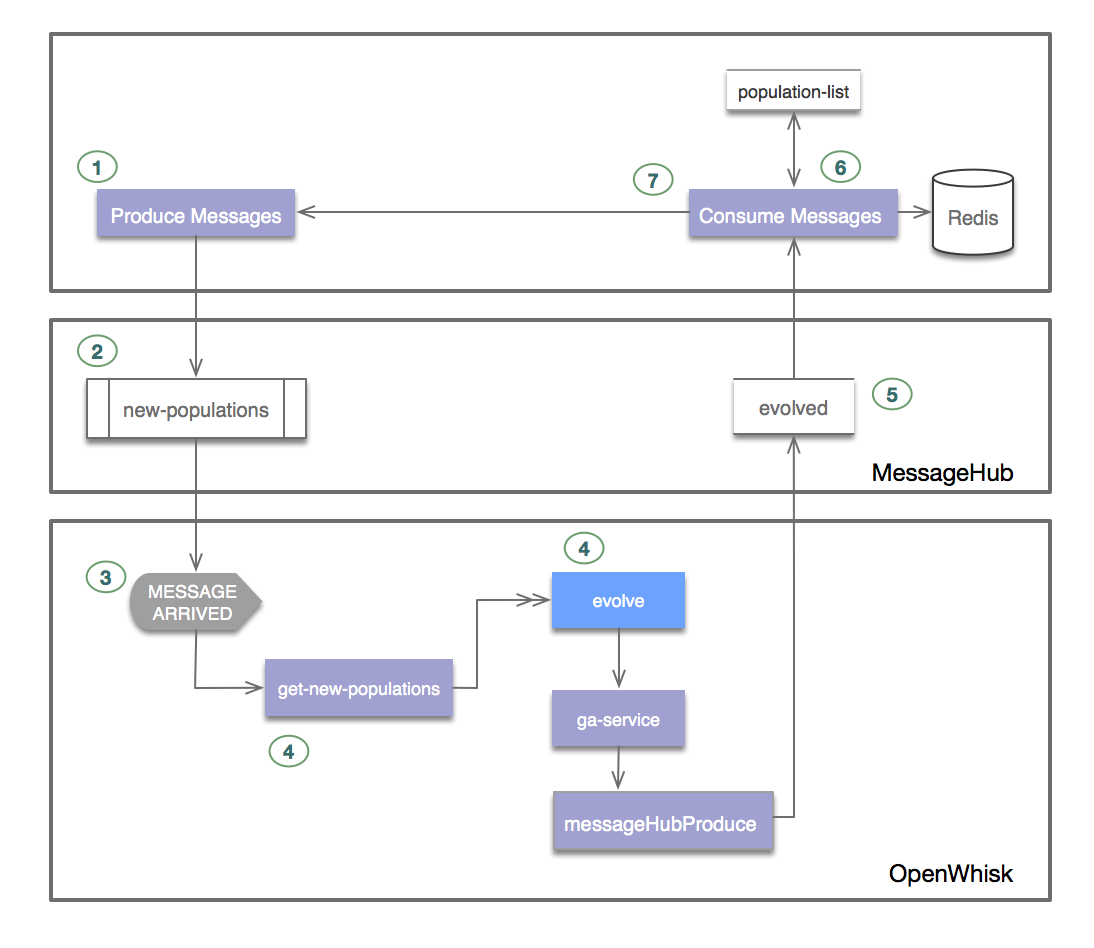
\includegraphics[width=0.95\textwidth]{img/kafka.png}
\caption{This chart shows the general picture of KafkEO, with message
  routes and the software components used for every part.}
\label{fig:kafkeo}
\end{figure*}
%
In the serverless, event based types of architectures we are going to
be targeting in this paper, there has been so far no work that we know
of. Similar setups including microservices have been employed by Salza et
al. \cite{salza2017ccube}; however, the serverless system adds a layer
of abstraction to event-based queuing systems such as the one employed
by Salza by reducing it to functions, messages and rules or
triggers. We will explain in detail these architectures in the next
section.

\section{Event based architectures and implementing evolutionary
  algorithms over them}
\label{sec:methods}
%
\begin{figure*}[h!tbp]
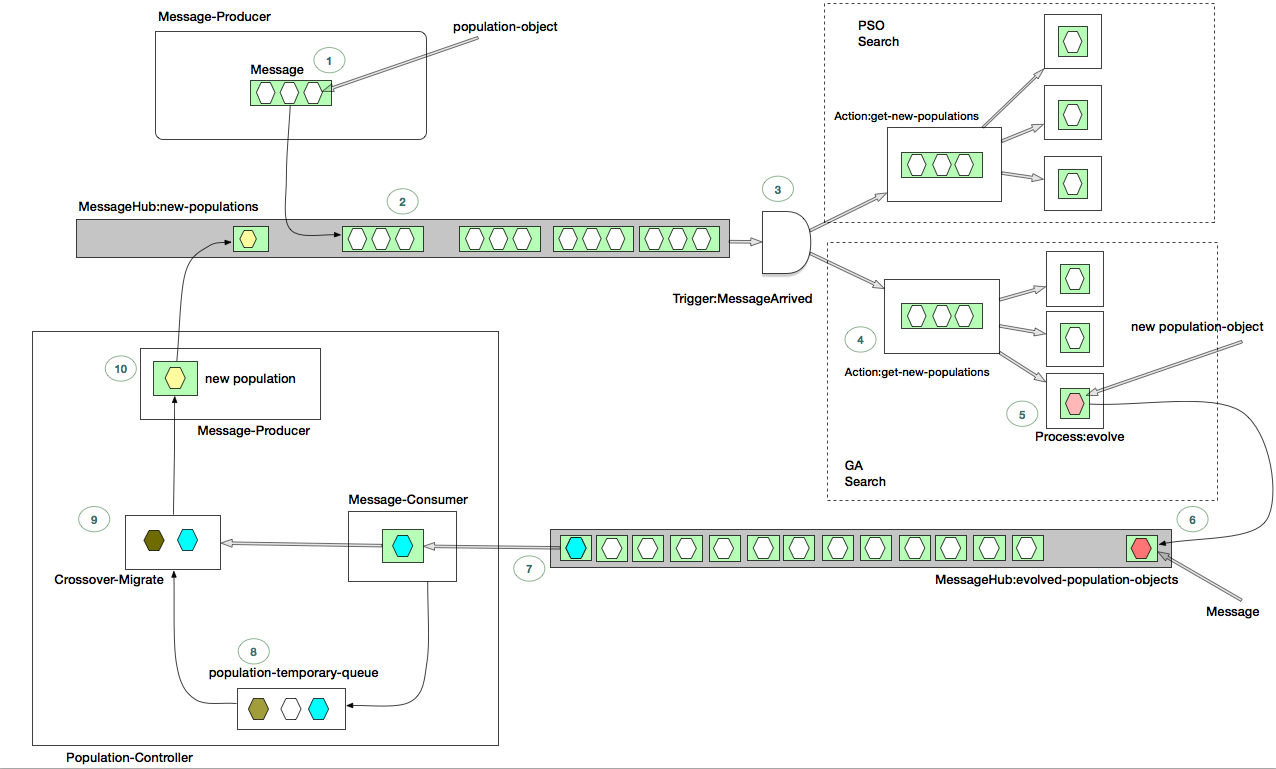
\includegraphics[width=0.95\textwidth]{img/kafkEO.png}
\caption{A flow diagram of KafkEO, showing message routes, MessageHub
  topics and the functions that are being used.}
\label{fig:kafkeo2}
\end{figure*}
%
The creation of virtualization and isolation mechanisms at many
different levels and the consequent granularization of architectures
has led to systems that are asynchronous and loosely coupled in what
is generally called a microservice architecture. These microservice
architectures share the common trait of consisting in several services
with a single concern, that is, providing a single processing value,
in many case stateless, and coupled using lightweight protocols such
as REST and messaging buses that carry information from every service
to the next. In this case, we are going to be using IBM's Bluemix
service, which includes OpenWhisk as a serverless framework and
MessageHub, also a vendor implementation of the Kafka messaging
service; this last one gives name to our framework, called KafkEO (EO
stands for Evolving Objects) and introduced in this paper.

The main reason why we have made this choice is availability of
resources, but also
the fact that all parts of the implementation are open source and can
be deployed in desktop machines or other cloud providers by changing
the configuration, as long as it is implemented using the same tools. It is also a good practice to implement free
% Maybe remove:  by simply changing names and IPs
% Is not a problem to do, but is litlle more than that.
% Clarified. Also to make clear that it's only if we keep using
% OpenWhisk and Kafka - JJ
software using free software, making it widely available to the
scientific community to create their own versions or to adapt it to
their own problems.

The layers and message flow in the application are shown in Figure
\ref{fig:kafkeo}, which also includes the evolutionary components. We
will focus for the time being in the general picture: a serverless
architecture using as a backbone a messaging service, which in this case
takes the shape of Kafka/MessageHub. These messages are produced and
consumed by a service, which can also store it in an external database
for its later use; in general, messaging systems are configured to
keep messages only for a certain amount of time, and they disappear
after that. Messaging queues are organized in {\em topics}; the
functions, hosted in OpenWhisk, execute {\em actions} triggered by the
arrival of new messages; these actions also produce new messages that
go back to the MessageHub to continue with the message loop.

The evolutionary algorithm mapped over this architecture, which we
call KafkEO, is represented in Figure \ref{fig:kafkeo2}. The main
design challenge is to try and map an evolutionary algorithm to a
serverless, and then stateless, architecture. That part is done in
points 1 through 5 of  \ref{fig:kafkeo2}. The beginning of the
evolution is triggered from outside the serverless framework (1) by
creating a series of populations, which we pack 3 to a message in the
{\em topic} {\sf new-populations}. The arrival of a new population
package sets off the {\sf MessageArrived} trigger, that is bound to
the actions that effectively perform evolution. In this case we
feature GA and PSO, although only GA has been implemented for this
paper. Any number of actions can be triggered in parallel, and new
actions can be triggered while others are still working; this phase is
then self-scaling and parallel by design.

Populations are extracted from the message and evolved for a number of
generations, generating another object in (6) that includes evolved
population and a series of metadata such as a flag that indicates
whether the solution has been found and the best individual. This
object is sent to another different message queue, {\sf
  evolved-population-objects}.

This queue is polled by a service outside the serverless framework,
{\sf Population-Controller}. This service needs to be stateful, since
it needs to wait until several populations are ready to mix them (in
step \#9) to produce a new population, that is the result of selection
and crossover between several populations coming from the {\sf
  evolved-population-objects} message queue. Eventually, these mixed
populations are returned to the initial queue to return to the {\em
  serverless} part of the application.

% consists essentially on a single function, a single topic
% in the MessageHub and a single kind of message, which includes a whole
% population along with metadata. The function performs a series of
% generations on the population, using a canonical algorithm with
% mutation and crossover. If it finds the solution, in our case, the
% minimum fitness, it sets a flag indicating it has found it so that it
% propagates to different instances of the population; in any case, it
% sends the whole evolved population as a message to the MessageHub, to
% be propagated to the other instantiations on the function.

This would be functionally equivalent to a sequential algorithm except
for the fact that, between two calls to the {\sf get-new-populations}
function, several 
population-messages have been received in the message queue. In fact,
every call the {\sf Crossover-migrate} function receives several populations, which
have to be merged to generate several new populations. This {\em merging} step
before starting evolution takes the place of the {\em migration} phase
and allows this type of framework to work in parallel, since several
instances of the function might be working at the exact same time; the
results of these instances are then received back by every one of the
instances.

In fact, this kind of system would be more functionally equivalent to
a pool-based architecture \cite{bollini1999distributed}, since the
queue acts as a pool from where populations are taken and where
evolved populations return. Actually, the pool becomes a {\em stream}
in this case, but in fact the pool also evolves, changing its
composition, and has a finite size just like the pool. Since
pool-based architectures have already proved they work with a good
performance, we might expect this type of architecture, being
functionally equivalent, to be at least just as efficient and the
latter, and better adapted to a cloud-native application.

In this phase where we are creating a proof of concent, there is a
single instance of this part. For the time being, it has not been
detected as a bottleneck, although eventually, when the number of
functions are working in parallel, it might become one. There are
several options for overcoming this problem, the easiest of which is
to add more instances of this {\sf Population-controller}. These
instances will act in parallel, processing the message queue at
different offsets and contributing to population diversity. This will
eventually have its influence in the results of the algorithm, so it
is better left as future work. 

Since we are running just a few functions, the amount of code of KafkEO
is quite small compared with other implementations. We use DEAP for
all the evolutionary functions, which are written in Python and
released in GitHub under the GPL license.



\section{Experiments and results}
\label{sec:res}

\section{Conclusions}
\label{sec:con}

% TO DO ------------------------------------------------

This paper is intended to introduce a simple proof of concept of a
serverless implementation of an evolutionary algorithm. As has been
explained, it needs a stateful {\em mixer} to be able to perform {\em
  migration} and mixing among populations. A straighforward first step
would be to paralellize this service so that it can respond faster to
incoming evolved populations; however, this scaling up should be done
by hand and a second step will be to make the architecture totally
serverless by using functions that perform this mixing in a stateless
way. This might have the secondary effect of simplifying the messaging
services to a single topic, and making deployment much easier by
avoiding the desktop or server back-end we are using now for that
purpose.

Other changes will go in the direction of testing the performance of
the system and computing the cost, so that we can increase the former
without increasing the latter. Since there is room for increasing
paralellism, we will try different ways of obtaining better
algorithmic results by making a parameter sensitivity analysis,
including population size, length of evolution runs, and other
algorithmic parameters.

Once those algorithmic baselines have been set, we will experiment
with different metaheuristics such as particle swarm optimization, or
even try for heterogeneous functions with different evolutionary
algorithm parameters, with the purpose of reducing the number of
parameters to set at the start.

On the implementation side, we will work on the automatic deployment
of this architecture to any free or vendor serverless implementation,
including maybe abstraction layers such as the {\tt serverless}
library. 




\begin{acks}

  The author would like to acknowledge the support of grants\\
  taking\\
  this\\
  much\\
  space\\

\end{acks}


\bibliographystyle{ACM-Reference-Format}
\bibliography{serverless}

\end{document}
